
%%%%%%%%%%%%%%%%%%%%%%%%%%%%%%%%%%%%%%%%%%%%%%%%%%%%%%%%%%%%%%%%%%%%%%%%%%%%%%%
%
% witseiepaper-2005.tex
%
%                       Ken Nixon (12 October 2005)
%
%                       Sample Paper for ELEN417/455 2005
%
%%%%%%%%%%%%%%%%%%%%%%%%%%%%%%%%%%%%%%%%%%%%%%%%%%%%%%%%%%%%%%%%%%%%%%%%%%%%%%%%

\documentclass[10pt,twocolumn]{witseiepaper}

%
% All KJN's macros and goodies (some shameless borrowing from SPL)
\usepackage{KJN}
\usepackage{graphicx}
\usepackage{booktabs,siunitx}
%multi-row
\usepackage{multirow}
\usepackage{multicol}
\newcommand{\RomanNumeralCaps}[1]
    {\MakeUppercase{\romannumeral #1}}
\usepackage{pdfpages}
\usepackage[normalem]{ulem}
\useunder{\uline}{\ul}{}

%
% PDF Info
%
\ifpdf
\pdfinfo{
/Title (INSTRUCTIONS AND STYLE GUIDELINES FOR THE PREPARATION OF FINAL YEAR LABORATORY PROJECT PAPERS : 2005 VERSION)
/Author (Ken J Nixon)
/CreationDate (D:200309251200)
/ModDate (D:200510121530)
/Subject (ELEN417/455 Paper Format, 2005)
/Keywords (ELEN417, ELEN455, paper, instructions, style guidelines, laboratory project)
}
\fi

%%%%%%%%%%%%%%%%%%%%%%%%%%%%%%%%%%%%%%%%%%%%%%%%%%%%%%%%%%%%%%%%%%%%%%%%%%%%%%%
\begin{document}


\title{\centering HEARTBEAT SOUND SEGMENTATION AND CLASSIFICATION}

\author{Boikanyo V. Radiokana
\thanks{School of Electrical \& Information Engineering, University of the
Witwatersrand, Private Bag 3, 2050, Johannesburg, South Africa}
}


%%%%%%%%%%%%%%%%%%%%%%%%%%%%%%%%%%%%%%%%%%%%%%%%%%%%%%%%%%%%%%%%%%%%%%%%%%%%%%%
%
\abstract{A heartbeat diagnostic system that consists mainly of preprocessing, segmentation and classification has been developed. Wavelet analysis is used for denoising and Shannon energy is used to find envelopes. For classification, ANN, SVM and XGBoost models were used. The system presented an accuracy of $80\%$ and $89\%$ for classifying normal heart sounds with SVM and XGBoost respectively. It is suggested that improving recording techniques and location of S1 and S2 will improve system performance.}

\keywords{Denoising, Segmentation, PCG (Phonocardiogram), Wavelet Analysis, }


\maketitle
\thispagestyle{empty}\pagestyle{empty}


%%%%%%%%%%%%%%%%%%%%%%%%%%%%%%%%%%%%%%%%%%%%%%%%%%%%%%%%%%%%%%%%%%%%%%%%%%%%%%%
%
\section{INTRODUCTION}
Cardiac auscultation remains to be the most popular yet challenging technique used by physicians to diagnose cardiovascular diseases (CVD's). Studies have shown that $22\%$, $26\%$ and $20\%$ of patients in the United States, Canada and England respectively were correctly diagnosed through auscultation \cite{1}. This technique has proven to be insufficient in diagnosing heart diseases since physicians still request unnecessary echocardiograms for reassurance \cite{strunic2007detection}, \cite{meziani2012analysis}. Echocardiograms are expensive and are normally done to avoid type \RomanNumeralCaps{2} errors \cite{strunic2007detection}. Type \RomanNumeralCaps{2} errors occur when a patient who has a CVD is sent home without any medical treatment. 

A heartbeat diagnostic system able to classify heart sounds into normal and diseased categories would help reduce the costs spent on unnecessary echocardiograms and also assist physicians to make well informed decisions during auscultation. This type of system would also be useful for home use by the general public by providing preliminary screening for CVD's. People would benefit from such a system as it will save them costs spent on unnecessary medical consultations.

This report presents a heartbeat sound segmentation and classification system capable of locating and segmenting heart sounds, primarily known as (lub and dub) or (S1 and S2) sounds from real-life recorded heart sounds. Segmentation is implemented in MATLAB using wavelet transforms amongst other methods for denoising. To detect peaks, Shannon energy is used. Machine learning models for classification and a user-interface are implemented in python.

Section 2 presents the background which outlines the project framework and Section 3 details the design methodology used. This is followed by implementation,test results, critical analysis of results and future recommendations respectively.

%%%%%%%%%%%%%%%%%%%%%%%%%%%%%%%%%%%%%%%%%%%%%%%%%%%%%%%%%%%%%%%%%%%%%%%%%%%%%%%
%
\section{BACKGROUND}

As mentioned above, this project aims to provide preliminary screening of heart diseases for both physicians and the general public for home use. This implies that the system should be applicable in real world surroundings with various background noises, some excessive depending on the environment.

According to literature \cite{debbal2008filtering}, \cite{gomes2012classifying}, the most common challenge with heart sounds that contain noise is segmentation and location of S1 and S2 sounds. Segmentation is considered a crucial step in the process of classifying heart sounds. It is therefore vital that heart sounds are detected as accurately as possible.

\subsection{Dataset}
\label{sec:dataset}
Only two datasets are used in this project, namely; Dataset-A and Dataset-B. Dataset-A is collected from the general public using an iStethoscope Pro iPhone app and Dataset-B was collected at a hospital using a digital stethoscope \cite{bentley2011pascal}. Dataset-A contains 124 recordings, each with a sampling frequency of 44100Hz and grouped into four categories: Normal, Murmur, Extra Heart Sound and Artifact. Dataset-B on the other hand contains 310 recordings, each with a sampling frequency of 4000Hz and grouped into three categories: Normal, Murmur and Extrasystole. Table \ref{tab:my_label} illustrates the distribution of data amongst the categories mentioned in each dataset.


\begin{table}[h!]
\centering
\caption{Dataset Distribution}
\begin{tabular}{llc}\hline%
\multicolumn {2}{c}{\textbf{Dataset} \textbf{ $\&$ Categories}}    & \textbf{Count}\\
&        & \\\hline%
Dataset-A    & Normal       & 31\\\cline{2-3}
& Murmur                      & 34\\\cline{2-3}
& Extra Hear Sound           & 19\\\cline{2-3}
& Artifact                   & 40\\\hline
Dataset-B    & Normal          & 200\\\cline{2-3}
& Murmur                     & 66\\\cline{2-3}
& Extrasystole                     & 44\\\hline
\end{tabular}
    \label{tab:my_label}
\end{table}
%%%%%%%%%%%%%%%%%%%%%%%%%%%
\subsection{Project Specifications and Requirements}
 A method that can successfully locate and segment S1 and S2 sounds from audio data must be implemented. This must be followed by a method to classify the heart sounds into normal and diseased categories. It is required that the project be carried out with only the audio data from Dataset-A and Dataset-B as stated above.

%%%%%%%%%%%%%%%%%%%%%%%%%%%
\subsection{Assumptions}
The project is executed with the assumption that the length of the audio recordings will be 30 seconds or less. It is also assumed that both Dataset-A and Dataset-B have integrity, in other words the audio data has been correctly placed within corresponding categories. 

%%%%%%%%%%%%%%%%%%%%%%%%%%%%%%
\subsection{Constraints}
The following constraints are to be considered when executing the project:

\begin{itemize}
    \item Segmentation must solely be based on the first and second heart sounds,                \textit{S1(lub)} and \textit{S2(dub)}.
    \item All audio data must be segmented on the basis of Normal heart sounds only.
    \item Only data from reference \cite{bentley2011pascal} can be used to execute the project due to ethics clearance.
    \item Audio heart sounds may only be in \textit{.wav} or \textit{.aif} format.
\end{itemize}

%%%%%%%%%%%%%%%%%%%%%%%%%%%%
\subsection{Success Criteria}

For the project to be deemed successful, it must fulfill all requirements stipulated in Section 2.2 and conform to all constraints stipulated in section 2.4. A normal classification accuracy of  equal to or higher than $77\%$ for Dataset-A and $46\%$ for Dataset-B will be highly desirable considering that existing solutions have an accuracy of up to 77\% and 46\% for the individual datasets.
%%%%%%%%%%%%%%%%%%%%%%%%%%%%%%%%%%%%%%%%%%%%%%%%%%%%%%%%%%%%%%%%%%%%%%%%%%%%%%%

\subsection{Related Works}
% Groch \textit{et al.} uses a microprocessor controlled heart sound gating device to identify S1 and S2 sounds individually using their timing relationships \cite{groch1992new}. The phonocardigrams are initially amplified as a consequence of being recorded with a microphone, coupled with get and put on a patients chest. The heart sounds are then filtered with a band-pass filter and its negative portions folded into its positive portions and enveloped. Peaks are identified using a Schmitt Trigger which generates a square wave when a peak is detected. This is followed by the identification of S1 and S2 sounds using the distinguishing features of systolic and diastolic periods.

As part of prepossessing, Angela \textit{et al.} and Iwata \textit{et al.} both downsample the signals down to 2000Hz to reduce noise \cite{iwata1980algorithm}, \cite{26}. Angela \textit{et al.} further uses wavelet decomposition with a fourth-level order six Daubechies filter to curb the remaining noisy components \cite{26}. The signal is then normalised to enable representation of data within a common scale, allowing effective analysis of feature relations.

Liang \textit{et al.} uses an eighth order Chebyshev Type \RomanNumeralCaps{1} lowpass filter with a cutoff frequency of 882Hz to get rid of noise \cite{liang1997heart}. The segmentation algorithm is based on a second-degree normalised Shannon energy which finds the envelope of the signal \cite{liang1997heart}. Peaks are identified using a threshold to avoid detecting very-low frequency signals. Incorrectly detected peaks are rejected using intervals between adjacent peaks as well as the energy of the peaks \cite{liang1997heart}. S1 and S2 sounds are identified by exploiting the fact that the diastolic period is larger than the systolic period. This method presents a segmentation accuracy of 93\%.

Majority of recent literature use wavelet transform and spectrogram to segment heart sounds  \cite{meziani2012analysis}, \cite{debbal2008filtering},\cite{liang1997heart}, \cite{deng2012robust}. It is suggested that wavelet analysis, in particular Discrete Wavelet Transform (DWT) yields better accuracy and is efficient in denoising heart sounds \cite{strunic2007detection}. The spectrogram on the other hand is mostly used to extract frequencies below 195Hz. This is a result of heart sounds generally being low frequency signals \cite{deng2012robust}.

As part of classification, Bentley constructs features based on the systolic and diastolic periods of the the heart sounds \cite{deng2012robust}. Gomes uses similar features to train  machine learning models and classifies the heart sounds with J48 (Decision Trees) and MLP (Multi Layer Perceptron) \cite{gomes2012classifying}. Strunic \textit{et al.} uses Artificial Neural Networks (ANN) to classify heart sounds which presents an accuracy of $85\pm7.4\%$ for simulated heart sounds \cite{strunic2007detection}. The accuracy decreases to $48\pm12.7\%$ when tested with recorded heart sounds. The drop in accuracy is caused by inaccurate detection and location of S1 and S2 sounds in recorded heart sounds.
%%%%%%%%%%%%%%%%%%%%%%%%%%%%%%%%%%%%%%%%%%%%%%%%%%%%%%%%%%%%%%%%%%%%%%%%%%%%%%%

\section{SYSTEM OVERVIEW}

The project is divided into 3 subsystems: Preprocessing, Segmentation and Classification respectively. Figure \ref{fig:flow} below illustrates the flow diagram which highlights the system overview. The input to the system is raw PCG signals from Dataset-A and Dataset-B.

\begin{figure}[h!]
    \centering
    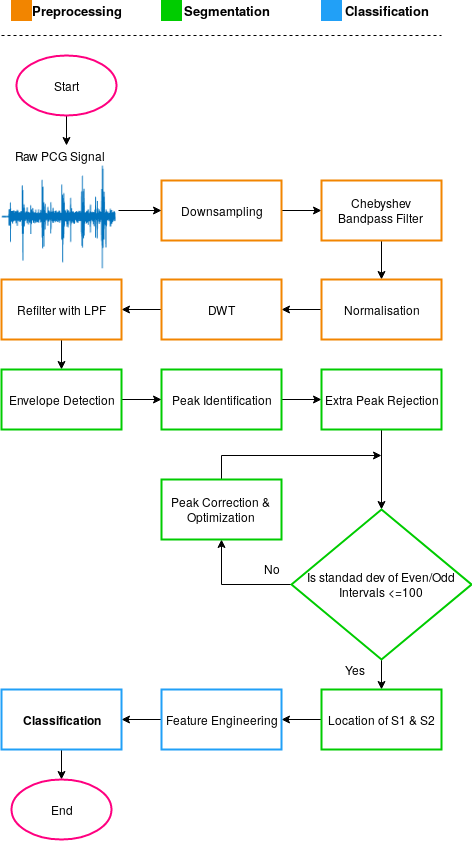
\includegraphics[width=8cm, height=12cm]{reportFDfinal.png}
    \caption{System Flow Diagram}
    \label{fig:flow}
\end{figure}
Preprocessing largely covers removing excessive noise from the PCG signals in order to condition the signals for segmentation. When the denoising process is completed, peaks are detected together with the location of S1 and S2 heart sounds. This is followed by construction of features important for classification, training of machine learning models and lastly classification of heart sounds into normal or diseased categories.

This paper will mainly focus on Preprocessing and Segmentation. Refer to \cite{elias} for a detailed explanation on Feature Extraction and Classification.
%%%%%%%%%%%%%%%%%%%%%%%%%%%%%%%%%%%%%%%%%%%%%%%%%%%%%%%%%%%%%%%%%%%%%%%%%%%%%%%
\section{IMPLEMENTATION}

\subsection{Preprocessing}
In Section \ref{sec:dataset} it is mentioned that the PCG signals are recorded in real-world situations, therefore there is a high possibility that the signals will contain artefacts and background noises. Noise can be caused by breathing sounds or fiddling with the stethoscope. Noisy signals make it impossible to analyse PCG signals, therefore, it is necessary to denoise the signals.

The first step to denoising the raw PCG signals is downsampling both datasets to 2000Hz. Downsampling compresses the data whilst retaining all the important information within the signal \cite{lavry2004sampling}. It also helps reduce high frequency components in the signal. The choice for 2000Hz sampling frequency abides by Nyquist Criterion and allows aliasing errors to be avoided.

Additionally a low bandpass Chebyshev filter of order 5 with a cut-off frequencies of 30Hz and 195Hz is applied to the downsampled signal. The filter is applied to further eliminate high frequency signals. Multiple researchers have chosen to apply filters with cut-off frequencies up to 600Hz  \cite{26}, \cite{deng2012robust}, \cite{rangayyan1987phonocardiogram}. They choose this band on the basis that murmurs contain frequencies up to 600Hz. The reason for choosing 195Hz as the upper cutoff frequency will be can be seen in Appendx \ref{app:pre}.

Before wavelet analysis can take place the PCG signal is normalised to obtain amplitudes ranging between $-1$ and 1 using Equation \ref{w}: 
\begin{equation}
    x_{norm}(i) = \frac{x_{f_{ds}}(i)}{max_{j}(|x_{f_{ds}}(j)|)}
    \label{w}
\end{equation}

where $x_{f_{ds}}$ is the signal obtained from applying the Chebyshev filter. 

\subsubsection{Wavelet Analysis}
\textcolor{white}{.................}\\
Denoising with only a bandpass filter is considered ineffective since some of the noisy signals overlap with some parts of the PCG signal \cite{39}. This creates a need to decompose the signal for analysis. Decomposition is implemented with a Discrete Wavelet Transform (DWT) which allows the analysis of the PCG signal in multiple frequency bands also known as multi-resolution analysis \cite{38}. In this project, a fifth-level DWT with a $7^{th}$ order Daubechies filter using a soft threshold is adopted. This wavelet is known as the mother wavelet.

The mother wavelet goes through various scaling and translation computations which yields a set of coefficients and functions called wavelets \cite{meziani2012analysis}, \cite{debbal2008filtering}. Equation \ref{mother} below shows the the DWT formula: 

\begin{equation}
    \psi_{(a,b)}(t) = \frac{1}{\sqrt{a}}\psi(\frac{t-b}{a})
    \label{mother}
\end{equation}

where \(\psi(t)\) is the mother wavelet and \(a\) and \(b\) are translation coefficients.
After decomposition and wavelet analysis the signals in the different bands are reconstructed using the coefficients. Coefficients found to have a value greater than the soft threshold are removed. Figure \ref{wavelet} illustrates the different levels ($d_{1}$-$d_{5}$) of the signals at different frequency bands as well as the approximated denoised signal ($a_{5}$). 

\begin{figure}[h!]
    \centering
    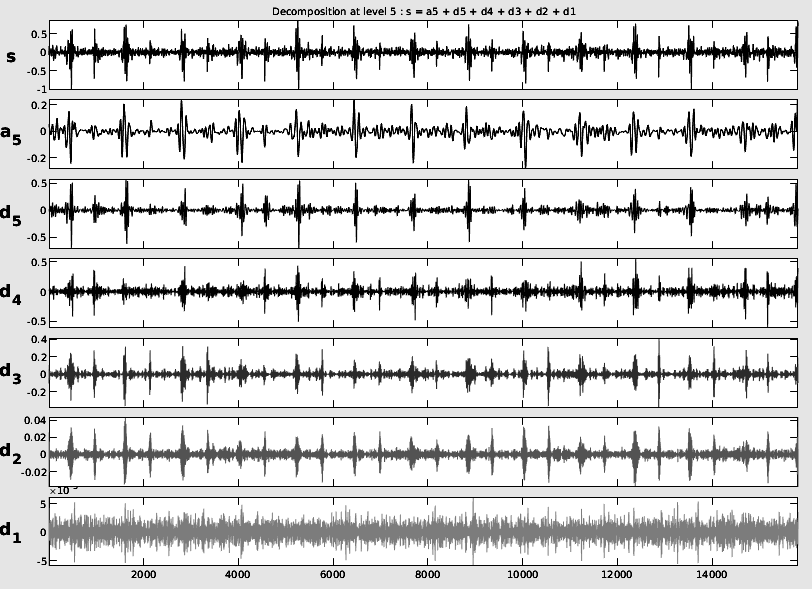
\includegraphics[width=8.5cm, height=10cm]{wavelet2.png}
    \caption{Level 5 DWT with $7^{th}$ order Daubechies Filter}
    \label{wavelet}
\end{figure}

The resultant denoised signal ($s$) is obtained by combining all the levels and approximation in Figure \ref{wavelet}. Equation \ref{dnny} shows how to generate the denoised signal.

\begin{equation}
 s = a5 + d5+d4+d3+d2+d1
 \label{dnny}
\end{equation}


To avoid unwanted frequency components after denoising with DWT, a low pass filter with a cutoff frequency of 195Hz is applied for refiltering.  Figure \ref{orig} and \ref{denoise} show the raw PCG signal and its FFT before and after preprocessing is applied.

\begin{figure}[h!]
    \centering
    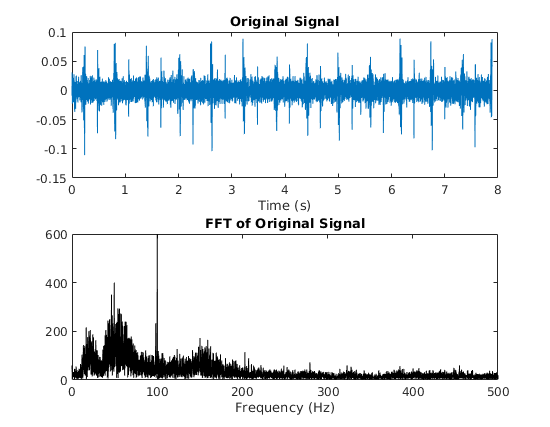
\includegraphics[scale=0.5]{orig.png}
    \caption{Raw PCG signal}
    \label{orig}
\end{figure}{}

\begin{figure}[h!]
    \centering
    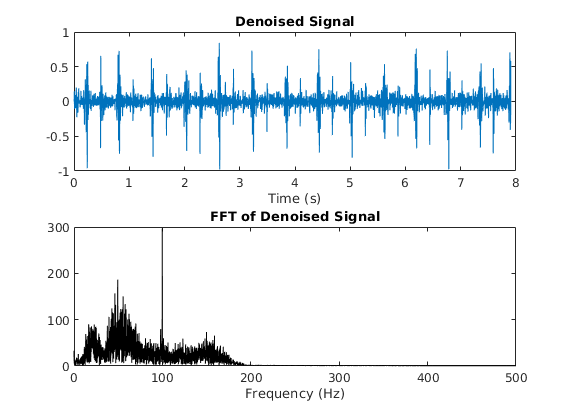
\includegraphics[scale=0.5]{denoise1.png}
    \caption{PCG Signal after Preprocessing}
    \label{denoise}
\end{figure}

\subsection{Segmentation}

\subsubsection{Envelope}
\textcolor{white}{.................}\\
After extensively denoising the PCG signal, a method to outline the envelope of the signal is implemented.
Envelopes are smooth, continuous functions that outline the extreme points of a signal \cite{29}.
The continuous functions make it relatively easy to identify peaks in a signal. The 
envelope is found using Shannon energy. Shannon energy is a popular method for threshold-based
peak identification methods \cite{11}. It is mostly preferred for
heartbeat sounds segmentation over other methods 
because of its exceptional performance. Shannon energy was adopted
it can attenuate low-amplitude noises and makes it easier to identify
low-intensity signals \cite{19}. The envelope of the signal was computed with Equation \ref{shannon} as follows:

\begin{equation}
    E = -x^2log(x^2)
    \label{shannon}
\end{equation}
\vspace{-1cm}
\subsubsection{Peak Identification}
\textcolor{white}{.................}\\
 Peaks are detected with a gradient method were derivatives of each point on the smooth signal is calculated. The points with derivatives that change from positive to negative are marked as peaks.

\subsubsection{Peak Rejection}
\textcolor{white}{.................}\\
Even with a substantial amount of denoising, noise is never removed completely. Therefore, some peaks might be wrongfully identified as heart sounds. It is crucial that all components that are not S1 and S2 sounds are removed, failure to do so will compromise the classification results.

To eliminate the wrongfully marked peaks, a threshold based on the third maximum peak is set. The threshold is set to $20\%$ of the third maximum peak. All peaks that are below this threshold are excluded.

\subsubsection{Peak Correction and Optimization}
\textcolor{white}{.................}\\
To verify if the peaks have been correctly detected, intervals between adjacent peaks are computed. The mean and standard deviation of odd and even intervals are calculated. If the standard deviation for either intervals is above 100 it means that there was an error in peak rejection. Two new thresholds are computed to correct this error, the upper and the lower threshold as seen in equation 1:

\begin{equation}
    t_{u,l} = |\mu\pm\sigma|
\end{equation}

where \(\mu\) is mean of the even or or odd intervals and \(\sigma\) is the standard deviation of the even or odd intervals.

An interval with a value higher than the upper-threshold suggests that a peak was missed and an interval with a value lower than the lower-threshold suggests that double peaks were detected. A missed peak is found by flagging the peaks between the corrupt interval. The two flagged peaks are used to map to the original signal before peak rejection. The peak with the largest amplitude between the two flagged peaks in the old signal will be now be marked as valid. 

As for the double detected peaks, the two peaks before the corrupt interval and the one after are flagged. The distance between the left most flagged peak and the two right most flagged peaks are calculated individually. The peak with a distance closest to the mean is taken and the other is dropped.

When peak correction is completed, the intervals are recalculated and the cycle continues until the condition is met, see Figure 1. Provided that the algorithm does not find any changes in consecutive iterations, it will exit the loop.

\subsubsection{Location of S1 and S2 Sounds}
\textcolor{white}{.................}\\
Location of S1 and S2 heart sounds is purely based on the fact that the diastolic period is larger than the systolic period. The largest interval is found and if it lies within the even intervals then all even peaks are marked as S1's, odd peaks as S2's and vice versa. The end result of preprocessing stages and segmentation can be seen in Appendix \ref{app:pre}.

\subsection{Feature Engineering and Classification}
After preprocessing and segmentation a total of 24 features are extracted. Only 21 features
are extracted from Dataset-A and 24 features from Dataset-B. From the located heart sounds, 10 features 
are extracted. The remaining features are from the frequency, cepstrum and wavelet domains \cite{elias}. The features are used to train and classify the heart sounds with the ANN, SVM and XGBoost machine learning
models.

\subsection{System GUI}
The user interface is implemnted in Python with PYQT5 application. It allows the user to see the end results of preprocessing, segmentation and classification results. The user has an option of choosing their desired model, see Appendix \ref{gee}, Figure \ref{gui}
%%%%%%%%%%%%%%%%%%%%%%%%%%%%%%%%%%%%%%%%%%%%%%%%%%%%%%%%%%%%%%%%%%%%%%%%%%%%%%%

\section{RESULTS}

Figure \ref{seg} depicts the segmentation accuracy of S1 and S2 heart sounds in the normal category for both Dataset-A and Dataset-B. Segmentation accuracy was calculated by counting the number of PCG signals which have a standard deviation smaller than 100 for both systolic and diastolic periods.
\begin{figure}[h!]
    \centering
    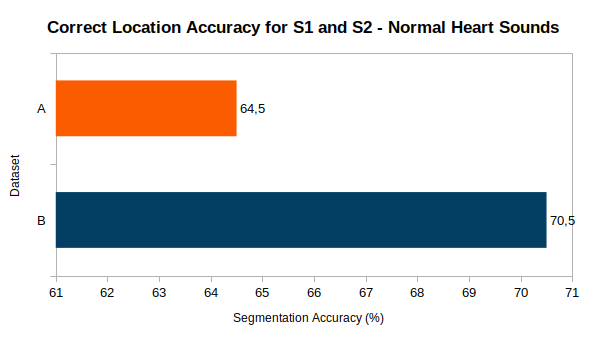
\includegraphics[scale=0.5]{elias.png}
    \caption{Segmentation Accuracy of Normal Heart Sounds in Dataset-A and Dataset-B}
    \label{seg}
\end{figure}{}

Table \ref{datasetA} and Table \ref{datasetB} show the performances for each dataset with the respective models as shown: 
\begin{table}[h!]
\centering
\caption{Classification Performance Dataset-A}
\label{datasetA}
\begin{tabular}{|c|c|c|c|c|}
\hline
\textbf{\begin{tabular}[c]{@{}c@{}}Class\\ (A)\end{tabular}} & \textbf{\begin{tabular}[c]{@{}c@{}}ANN\\ (\%)\end{tabular}} & \textbf{\begin{tabular}[c]{@{}c@{}}SVM\\ (\%)\end{tabular}} & \textbf{\begin{tabular}[c]{@{}c@{}}XGB\\ (\%)\end{tabular}} & \textbf{\begin{tabular}[c]{@{}c@{}}Liter-\\ ature(\%)\end{tabular}} \\ \hline
Normal & 27 & 80 & 71 & 45 \\ \hline
Murmur & 88 & 78 & 86 & 31 \\ \hline
ExtraHS & 67 & 25 & 57 & 11 \\ \hline
Artifact & 100 & 57 & 50 & 58 \\ \hline
\begin{tabular}[c]{@{}c@{}}Overall\\ Accuracy\end{tabular} & \textbf{81} & \textbf{64} & \textbf{68} & \textbf{46} \\ \hline
\end{tabular}
\end{table}

\begin{table}[h!]
\centering
\caption{Classification Performance Dataset-B}
\label{datasetB}
\begin{tabular}{|c|c|c|c|c|}
\hline
\textbf{\begin{tabular}[c]{@{}c@{}}Class\\ (B)\end{tabular}} & \textbf{\begin{tabular}[c]{@{}c@{}}ANN\\ (\%)\end{tabular}} & \textbf{\begin{tabular}[c]{@{}c@{}}SVM\\ (\%)\end{tabular}} & \textbf{\begin{tabular}[c]{@{}c@{}}XGB\\ (\%)\end{tabular}} & \textbf{\begin{tabular}[c]{@{}c@{}}Liter-\\ ature(\%)\end{tabular}} \\ \hline
Normal & 80 & 77 & 89 & 78 \\ \hline
Murmur & 90 & 87 & 75 & 37 \\ \hline
Extrasys & 15 & 0 & 17 & 17 \\ \hline
\begin{tabular}[c]{@{}c@{}}Overall\\ Accuracy\end{tabular} & \textbf{80} & \textbf{78} & \textbf{79} & \textbf{77} \\ \hline
\end{tabular}
\end{table}

Results for feature importance can be seen in figure \ref{fig:boost}, Appendix \ref{app:features}.
%%%%%%%%%%%%%%%%%%%%%%%%%%%%%%%%%%%%%%%%%%%%%%%%%%%%%%%%%%%%%%%%%%%%%%%%%%%%%%%
\section{CRITICAL ANALYSIS OF RESULTS}

From observation of results, it can be seen that S1 and S2 heart sounds were
mostly incorrectly identified in Dataset-A. One of the major reasons for this is the high
inclusion of a wide variety of background noises since it was recorded by the general public. This makes it difficult to segment the heart sounds since most noisy components overlap with the heart sounds. Another reason to explain why the segmentation accuracy of both datasets is not high is the high intensity of murmurs which also overlaps with the heart sounds, making it impossible to differentiate between S1 and S2 sounds and murmurs.

The sudden release of the stethoscope from the patient while recording greatly affects the segmentation results since the first and last peaks have to be excluded from analysis. This means that valuable information is lost.

As seen in figure \ref{fig:boost}, Appendix \ref{app:features}, it is shown that out of the top 6 most important features, 4 are computed from segmentation results. This implies that segmentation greatly affects classification, therefore: accurate segmentation results in a high classification accuracy. 

The best performing machine learning models for classifying normal heart sounds in Dataset-A and Dataset-B according to Table 2 and 3 is SVM and XGBoost with an accuracy of $89\%$ and $80\%$ respectively. For murmurs, ANN performed best in both datasets with an accuracy of $88\%$ for Dataset-A and $90\%$ for dataset B. One major flaw identified in this project is the inability of all models to classify extrasystole heart sounds in Dataset-B. The reason for obtaining these results is the unequal distribution of data amongst the categories. This means that the models are mostly acquainted with normal heart sounds and murmurs rather than extrasystoles. After careful study of the heart sounds, it was observed that the extrasystole class has similar characteristics to normal heart sounds, making it difficult to distinguish between the two \cite{bentley2011pascal}.

With the above mentioned, it can be concluded that the system met the success criteria stipulated in Section 2.5.
%%%%%%%%%%%%%%%%%%%%%%%%%%%%%%%%%%%%%%%%%%%%%%%%%%%%%%%%%%%%%%%%%%%%%%%%%%%%%%%
%
\section{RECOMMENDATIONS FOR FUTURE WORK}
To achieve better segmentation results, recording techniques can be improved as well as better segmentation techniques. Classification can also be improved by training models with an equally distributed dataset to avoid having biased models. Better ways of distinguishing extrasystoles and extra heart sounds need to be developed.

%%%%%%%%%%%%%%%%%%%%%%%%%%%%%%%%%%%%%%%%%%%%%%%%%%%%%%%%%%%%%%%%%%%%%%%%%%%%%%%%
\section{CONCLUSION}

A method to segment and classify heart sounds into normal and diseased categories has been successfully developed and implemented. Wavelet analysis and Shannon energy are used to denoise the PCG signal and generate the envelope respectively. Methods to improve location of S1 and S2 have been proposed. The system presented an segmentation accuracy of $64.5\%$ and $70.5\%$ for Dataset A and B respectively. Machine learning models used for classification include ANN, SVM and XGBoost. SVM and XGBoost presented a classification accuracy of $80\%$ and $89\%$ for normal heart sounds for Dataset A and B respectively. 

%%%%%%%%%%%%%%%%%%%%%%%%%%%%%%%%%%%%%%%%%%%%%%%%%%%%%%%%%%%%%%%%%%%%%%%%%%%%%%%%

\section*{ACKNOWLEDGEMENTS}
The author would like to thank Ms Ellen De Mello Koch for her guidance and Elias Sepuru for his contribution to the project and being a great partner.
%%%%%%%%%%%%%%%%%%%%%%%%%%%%%%%%%%%%%%%%%%%%%%%%%%%%%%%%%%%%%%%%%%%%%%%%%%%%%%%%



%%%%%%%%%%%%%%%%%%%%%%%%%%%%%%%%%%%%%%%%%%%%%%%%%%%%%%%%%%%%%%%%%%%%%%%%%%%%%%%
%
%\nocite{*}
% \newpage

\bibliographystyle{witseie}
\bibliography{sample}

\newpage
\onecolumn
\appendices

%%%%%%%%%%%%%%Group Reflection%%%%%%%%%%%%%%%%%%%%%%
\section{Reflection on Group Work}

\subsection{\textbf{Introduction}}
In this document, the work division amongst the members of the group, challenges encountered as well as the author's personal reflection of working in a group is presented.

\subsection{\textbf{Work Division}}
Initially me and my partner, Elias Sepuru preferred to work together to ensure that both team members have a common and solid understanding of the project requirements, specifications and dataset. The initial plan was that both members will try different approaches for the same section and the technique that yields the best results will be chosen. However, due to limited time and complexity of some methods, it was decided that working in parallel will not be feasible. This required us to go back to the drawing board to restructure the work division. The division of tasks can be seen in Table 1 below. This does not strictly suggest that the members mentioned in the respective tasks did all the work alone. The members fairly distributed work amongst themselves and if anyone needed help the other member was always ready to help.

\begin{table}[h!]
\centering
\caption{Work Division}
\label{undefined}
\begin{tabular}{|l|l|}
\hline
\textbf{Task} & \textbf{Team Member} \\ \hline
Preprocessing & Boikanyo \\ \hline
Segmentation & Boikanyo \\ \hline
Feature Extraction & Elias \\ \hline
Classification & Elias \\ \hline
GUI Front-end & Boikanyo \\ \hline
GUI Back-end & Elias \\ \hline
GUI Integration & Boikanyo and Elias \\ \hline
Project Poster & Boikanyo and Elias \\ \hline
\end{tabular}
\end{table}

\subsection{\textbf{Challenges Encountered}}
The only challenges we encounted in the first few weeks was to accurately locate S1 and S2 sounds and machine learning optimization. We realised that if these tasks are not executed well the success of the project will be compromised. We were forced to invest most of our time in perfecting these sections which turned out well in the end.

\subsection{\textbf{Personal Reflection on Group Work}}
Elias Sepuru and I have previously worked together on school projects and labs. We are well aware of each others work ethic, strengths and weaknesses. We worked well together throughout the project because we share a similar work ethic, interests and goals when it comes to academic work. One of the most valuable skills I have learned while working with Elias is to effectively communicate my ideas and thoughts. This enabled both of us to look at things from a different perspective and to also foresee challenges that we might encounter. We are always ready to tackle any work assigned to us which  helped with the progress of the project. One strength but mostly a weakness that we both have is that we are perfectionists. We always take more time to complete tasks than anticipated which results in us working close to the deadline. In future this is one of the things I would like to improve about myself. One of the things I enjoyed about working in a group is that I did not have to do all the work alone. Elias's positive attitude always motivated me to work hard despite the challenges we encountered. All in all I am proud of the work we put in this project as well as the quality of work we both produced.

\subsection{\textbf{Conclusion}}
The work was equally divided amongst team members and the project was successfully completed. Communication and being aware of team players work ethic greatly affects the success of the project.
%%%%%%%%%%%%%%Lab specifications%%%%%%%%%%%%%%%%%%%%%%
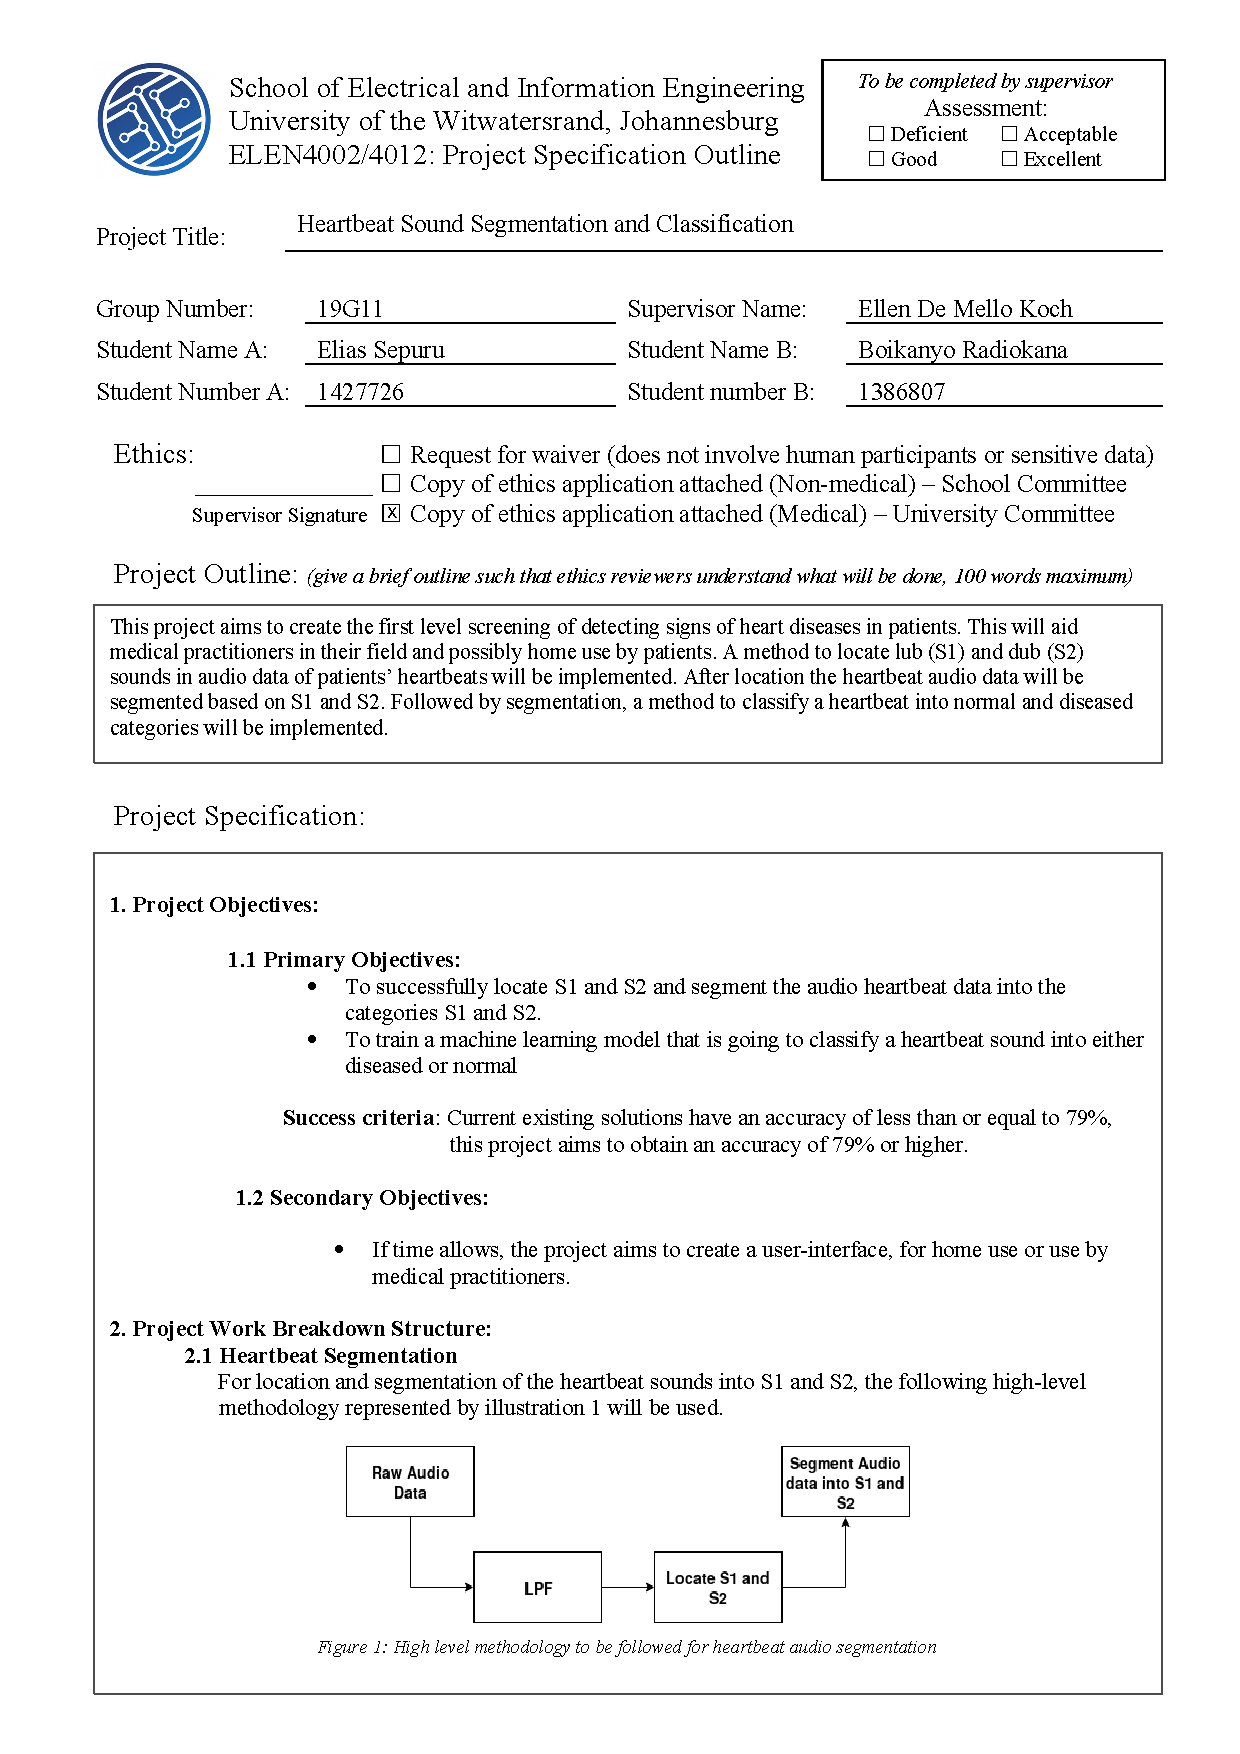
\includepdf[scale=0.94,pages=1,pagecommand={\section{Project Specification}\thispagestyle{empty}},fitpaper=true]{labspecs.pdf}
\includepdf[scale=0.94,pages=2,pagecommand={\thispagestyle{empty}},fitpaper=true]{labspecs.pdf}

%%%%%%%%%%%%%%Project Plan%%%%%%%%%%%%%%%%%%%%%%

\includepdf[scale=0.94,pages=1,pagecommand={\section{Project Plan}\thispagestyle{empty}},fitpaper=true]{projectPlan.pdf}

\includepdf[scale=0.94,pages=2-6,pagecommand={\thispagestyle{empty}},fitpaper=true]{projectPlan.pdf}


%%%%%%%%%%%%%%Clearance Certificate%%%%%%%%%%%%%%%%%%%%%%
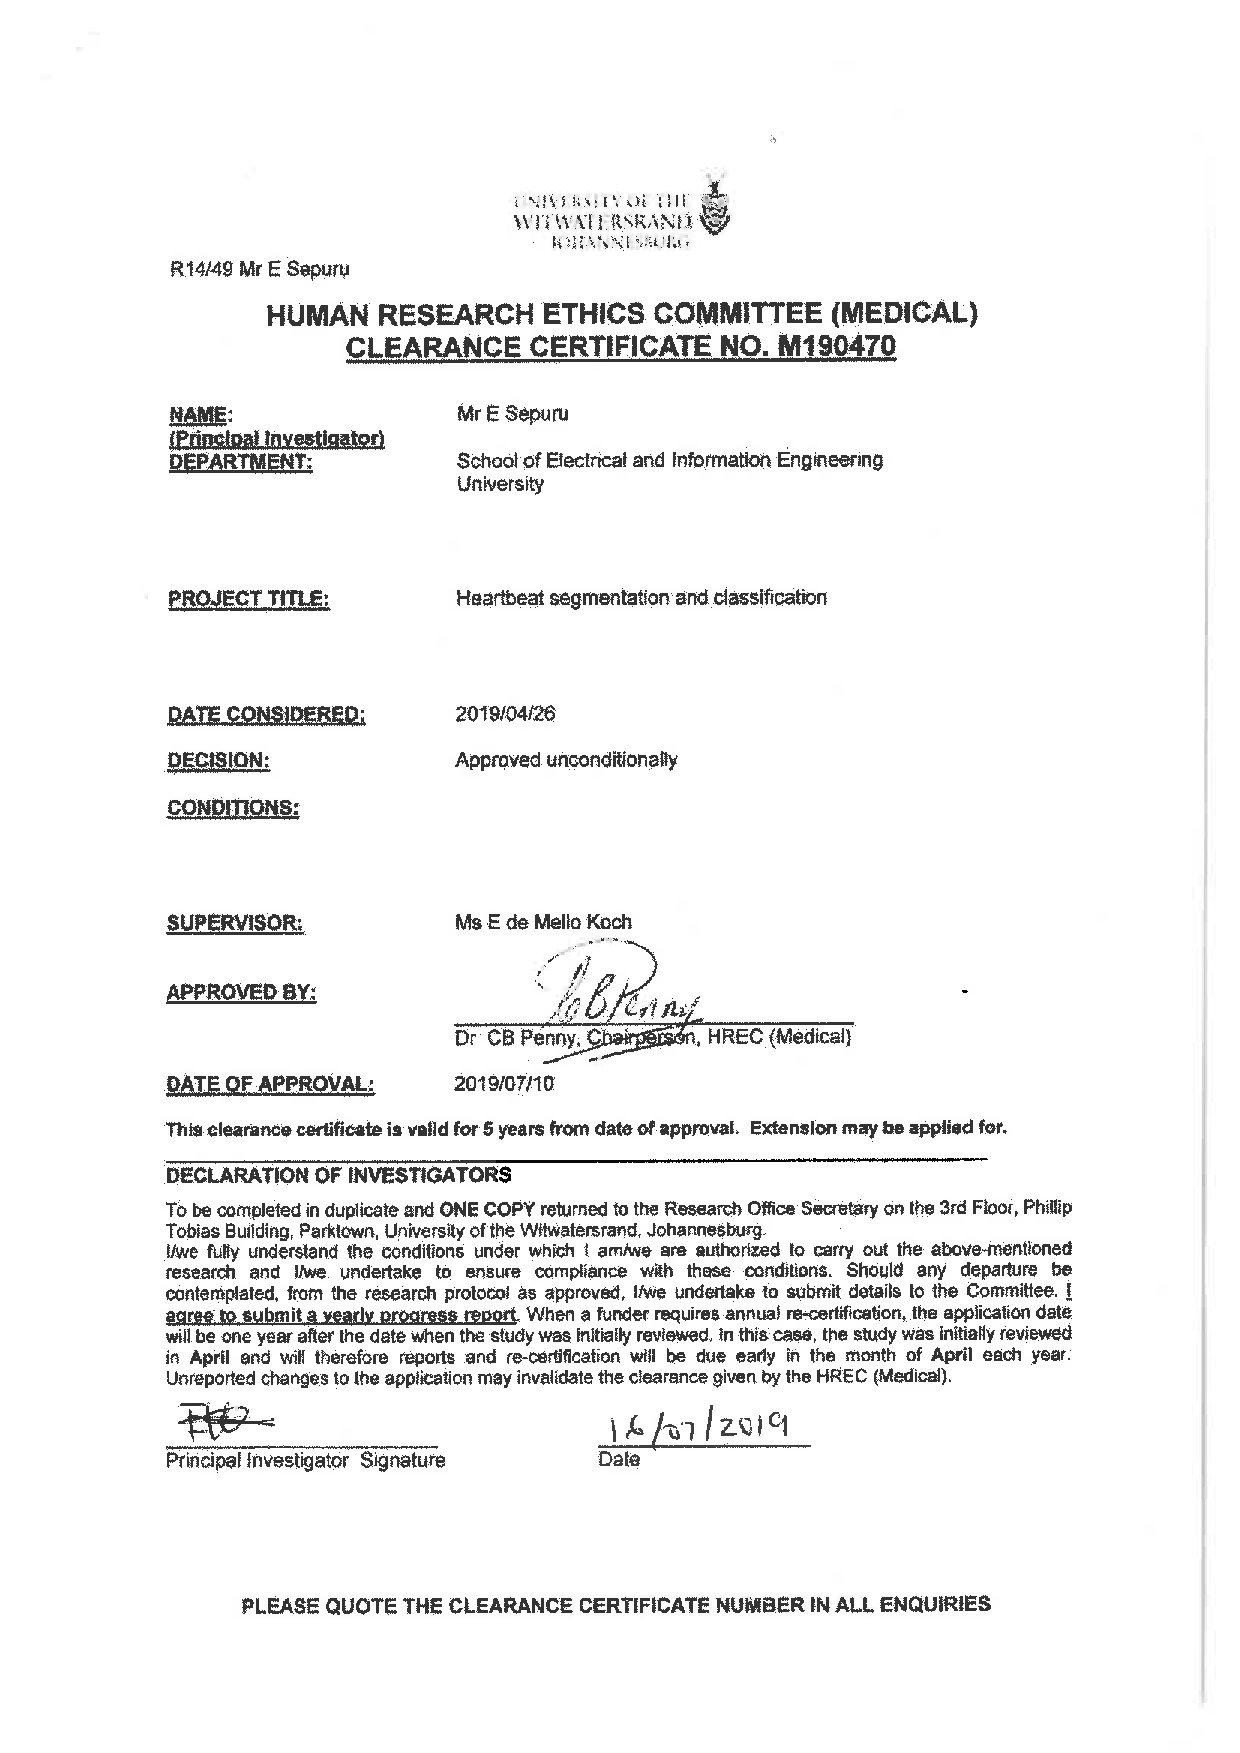
\includepdf[scale=0.94,pages=1,pagecommand={\section{ETHICS CLEARANCE CERTIFICATE}\thispagestyle{empty}},fitpaper=true]{clearanceCertificate.pdf}


%%%%%%%%%%%%%%%%%%%%%55
\twocolumn
\section{Preprocessing and segmentation}
\label{app:pre}
The following figures show the end result of each an every process in the system, from preprocessing all the way to segmentation.

Figure \ref{fig:6} shows the raw PCG signal before preprocessing. It is evident that most energy is concentrated below 200Hz. No valuable features can be extracted above 200Hz. Therefore filters with cutoff frequencies equal to 195Hz will work.
\begin{figure}[h!]
    \centering
    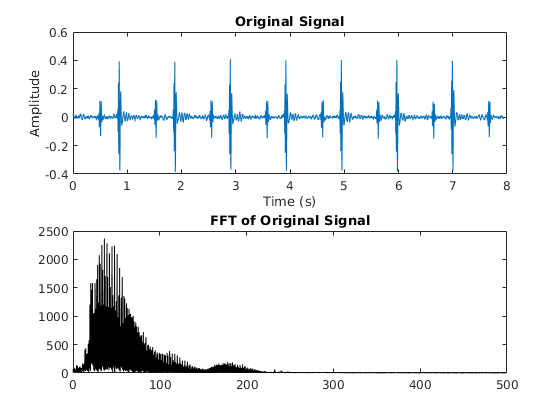
\includegraphics[scale = 0.6]{1.png}
    \caption{Raw audio PCG Signal}
    \label{fig:6}
\end{figure}{}

Figure \ref{fig:7} shows the PCG signal after preprocessing.
\begin{figure}[h!]
    \centering
    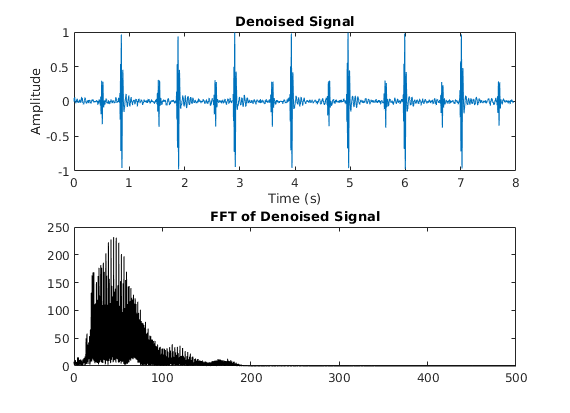
\includegraphics[scale = 0.6]{2.png}
    \caption{Denosed Signal}
    \label{fig:7}
\end{figure}{}

Figure \ref{fig:8} shows the envelope of the signal using Shannon energy.
\begin{figure}[h!]
    \centering
    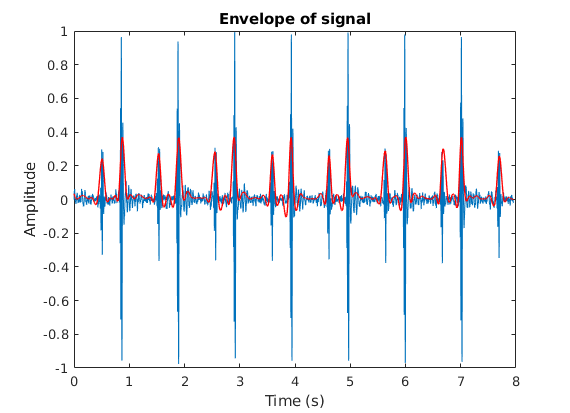
\includegraphics[scale = 0.55]{3.png}
    \caption{Envelope of Signal}
    \label{fig:8}
\end{figure}{}

Figure \ref{fig:9} shows the peaks detected using gradient method. Some of the peaks detected are noisy components.
\begin{figure}[h!]
    \centering
    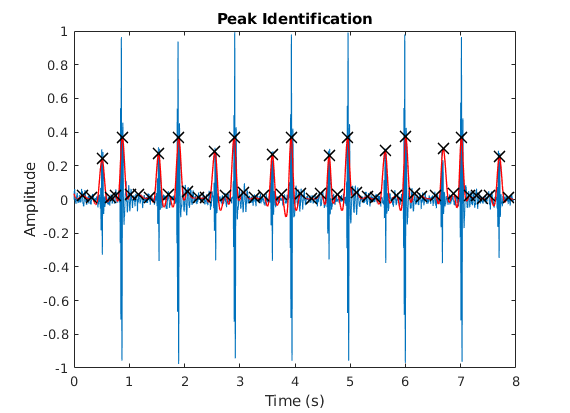
\includegraphics[scale = 0.55]{4.png}
    \caption{Peak Identification}
    \label{fig:9}
\end{figure}{}

Figure \ref{fig:10} shows the PCG signal after peak rejection, correction and optimization.
\begin{figure}[h!]
    \centering
    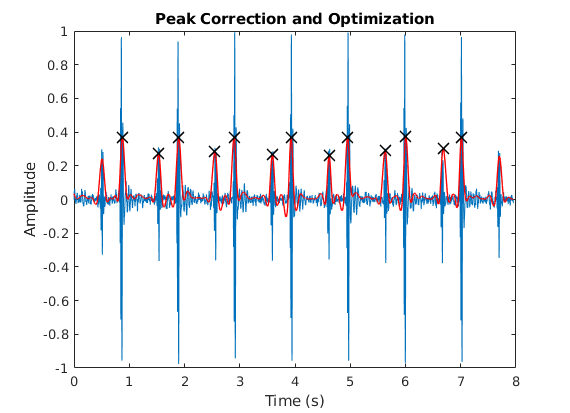
\includegraphics[scale = 0.55]{5.png}
    \caption{Peak Correction and Optimization}
    \label{fig:10}
\end{figure}{}

\twocolumn
\newpage
%%%%%%%%%%%%%Additional Work%%%%%%%%%%%%%%%%%%%%%%
\section{Extracted Features}
\label{app:features}
Table \ref{tab:tfeat}, \ref{tab:wav}, \ref{fre} and  \ref{cep} shows all features  extracted from the time ,frequency domain, wavelet analysis and cepstrum domain.

\begin{table}[h!]
\caption{Features from the time-domain}
\label{tab:tfeat}
\begin{tabular}{|l|l|}
\hline
\multicolumn{1}{|c|}{\textbf{Feature}} & \multicolumn{1}{c|}{\textbf{Description}} \\ \hline
\multicolumn{1}{|c|}{stdS1} & \multicolumn{1}{c|}{\label{t:s1}Standard deviation of systolic period.} \\ \hline
\multicolumn{1}{|c|}{stdS2} & \multicolumn{1}{c|}{\label{t:s2}Standard deviation of diastolic period.} \\ \hline
meanS1 & Mean of systolic period. \\ \hline
meanS2 & Mean of diastolic period. \\ \hline
maxstdS1 & \begin{tabular}[c]{@{}l@{}}Standard deviation of systolic period \\ after dropping the largest interval.\end{tabular} \\ \hline
maxstdS2 & \begin{tabular}[c]{@{}l@{}}Standard deviation of diastolic period \\ after dropping the largest interval.\end{tabular} \\ \hline
mmstdS1 & \begin{tabular}[c]{@{}l@{}}Standard deviation of systolic period \\ after dropping the largest and smallest\\ intervals.\end{tabular} \\ \hline
mmstdS2 & \begin{tabular}[c]{@{}l@{}}Standard deviation of diastolic period \\ after dropping the largest and smallest\\ intervals.\end{tabular} \\ \hline
prRatio & \begin{tabular}[c]{@{}l@{}}\label{t:pr}Ratio of the total number of peaks left\\ after Peak Rejection over\\ the length of the audio file\end{tabular} \\ \hline
pcRatio & \begin{tabular}[c]{@{}l@{}}\label{t:pc}Ratio of the total number of peaks left\\ after Peak Correction over \\ peaks from Peak Rejection.\end{tabular} \\ \hline
\end{tabular}
\end{table}

\begin{table}[h!]
\caption{Features extracted from DWT}
\label{tab:wav}
\begin{tabular}{|c|l|}
\hline
\textbf{Feature} & \multicolumn{1}{c|}{\textbf{Description}} \\ \hline
rebuildError & \begin{tabular}[c]{@{}l@{}}Average difference between the PCG\\ signal before denoising and the PCG\\ signal after denoising.\end{tabular} \\ \hline
stdWavelet & \begin{tabular}[c]{@{}l@{}}Standard deviation of the approxim-\\ ation of a  $6^{th}$ level db6 DWT \\ \\ of the preprocessed PCG signals.\end{tabular} \\ \hline
\multicolumn{1}{|l|}{meanWavelet} & \begin{tabular}[c]{@{}l@{}}Mean of the approximation of a $6^{th}$\\ level db6 DWT of the preprocessed\\ PCG signals.\end{tabular} \\ \hline
\end{tabular}
\end{table}

\begin{table}[]
\centering
\caption{Features  extracted  from  the  frequency-domain}
\label{fre}
\begin{tabular}{|c|l|}
\hline
\textbf{Feature} & \multicolumn{1}{c|}{\textbf{Description}} \\ \hline
stdFFTSHA & \begin{tabular}[c]{@{}l@{}}Standard deviation of the identified\\ peaks in the [180 190] Hz band.\end{tabular} \\ \hline
lenFFTSHA & \begin{tabular}[c]{@{}l@{}}Count of qualifying peaks identified\\ in the [180 190] Hz band.\end{tabular} \\ \hline
\begin{tabular}[c]{@{}c@{}}stdlen\\ FFTSHA\end{tabular} & \begin{tabular}[c]{@{}l@{}}Ratio of stdFFTSHA over\\ lenFFTSHA.\end{tabular} \\ \hline
lenstdFFTSHA & \begin{tabular}[c]{@{}l@{}}Ratio of lenFFTSHA over \\ stdFFTSHA.\end{tabular} \\ \hline
\multicolumn{1}{|l|}{posFFT} & \begin{tabular}[c]{@{}l@{}}Count of peaks from Shannon\\ Energy of FFT.\end{tabular} \\ \hline
\end{tabular}
\end{table}

\begin{table}
\caption{Features extracted from Cepstrum}
\label{cep}
\begin{tabular}{|c|l|}
\hline
\textbf{Feature} & \multicolumn{1}{c|}{\textbf{Description}} \\ \hline
stdPCA1 & \begin{tabular}[c]{@{}l@{}}Standard deviation of the first \\ \\ PCA vector.\end{tabular} \\ \hline
meanPCA1 & Mean of the first PCA vector. \\ \hline
stdPCA2 & \begin{tabular}[c]{@{}l@{}}Standard deviation of the second\\ PCA vector.\end{tabular} \\ \hline
meanPCA2 & Mean of the second PCA vector. \\ \hline
\multicolumn{1}{|l|}{stdPCA3} & \begin{tabular}[c]{@{}l@{}}Standard deviation of the third\\ PCA vector.\end{tabular} \\ \hline
\multicolumn{1}{|l|}{meanPCA3} & Mean of the third PCA vector. \\ \hline
\end{tabular}
\end{table}

\newpage
Figure \ref{fig:boost} shows the features in all the tables presented above in the order of the most important to the least important. From the top 6, 4 of the features are from the results obtained from segmentation.
\begin{figure}[h!]
    \centering
    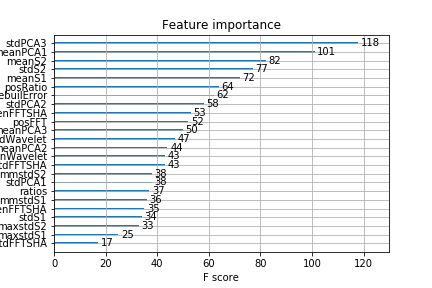
\includegraphics[scale=0.6]{boost.png}
    \caption{Feature Importance}
    \label{fig:boost}
\end{figure}{}

%%%%%%%%%%%%%%%%%%%%%%%%%%%%%%%%%%%%%%%%%%%%%%%%%%%
\onecolumn
\newpage
\section{System GUI}
\label{gee}
The following figure shows the implemented user interface. The user interface is implemented in python using PYQT5. It allows the user to choose their desired model from ANN, SVM or XGBoost. The pictures shown in the interface are raw audio data before preprocessing, after and the end result of segmentation. When a model is evaluated, the classification results are presented together with the confidence of the model.


\begin{figure}[h!]
    \centering
    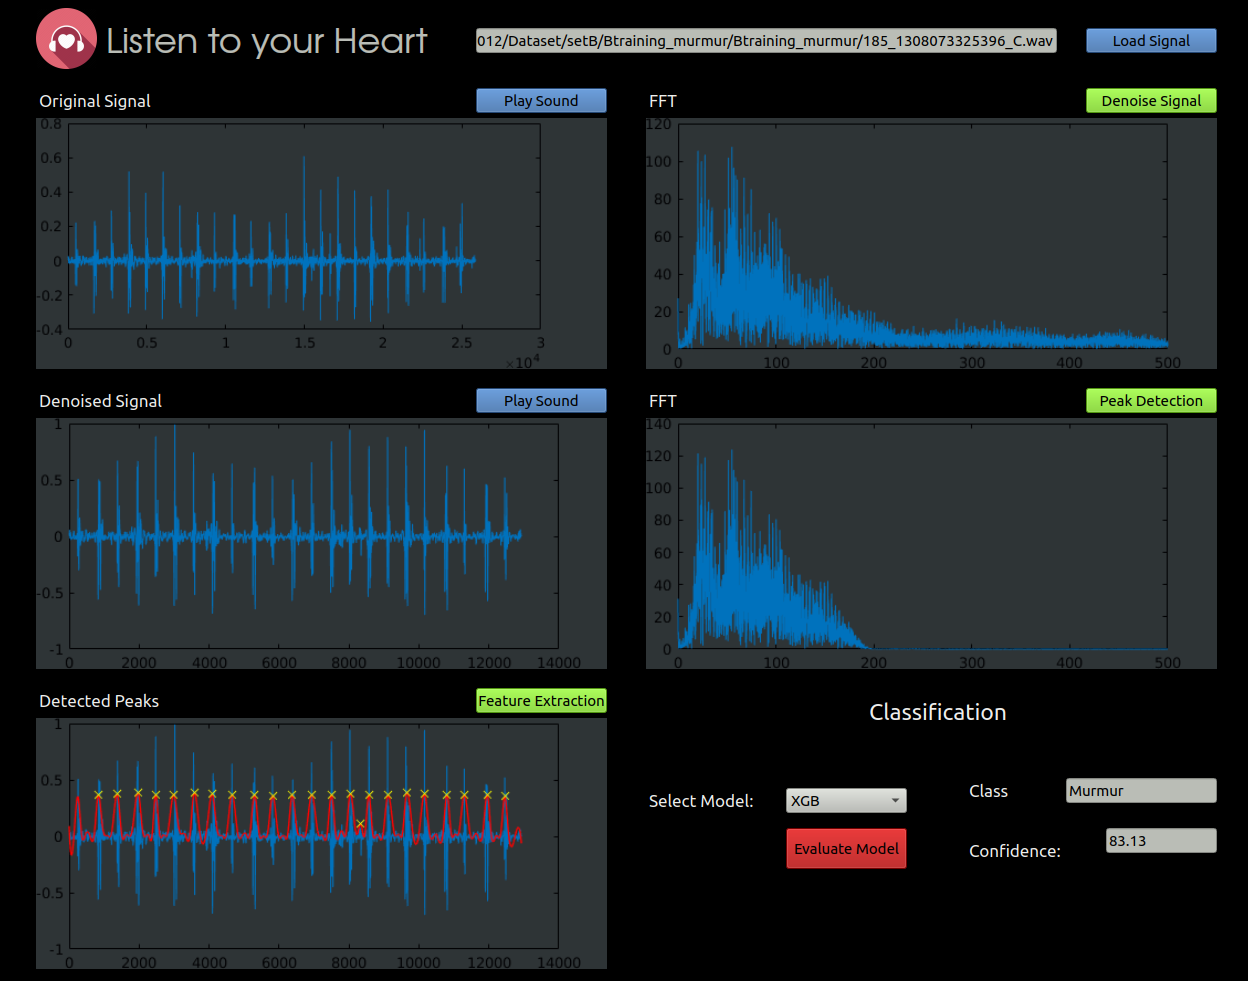
\includegraphics[width = 18cm, height = 20cm] {GUI.png}
    \caption{System User-interface}
    \label{gui}
\end{figure}{}
\newpage
\onecolumn

%%%%%%%%%%%%%%MEETINGS CLEARANCE%%%%%%%%%%%%%%%%%%%%%%

\includepdf[scale=0.94,pages=1,pagecommand={\section{MEETINGS MINUTES}\thispagestyle{empty}},fitpaper=true]{minutes.pdf}

\includepdf[scale=0.94,pages=2-32,pagecommand={\thispagestyle{empty}},fitpaper=true]{minutes.pdf}


%{\tiny \vfill \hfill \today \hspace{5mm} witseie-paper-2003.\TeX}
\end{document}



" vim: ts=4
" vim: tw=78
" vim: autoindent
" vim: shiftwidth=4
